% Options for packages loaded elsewhere
\PassOptionsToPackage{unicode}{hyperref}
\PassOptionsToPackage{hyphens}{url}
\PassOptionsToPackage{dvipsnames,svgnames*,x11names*}{xcolor}
%
\documentclass[
]{article}
\usepackage{lmodern}
\usepackage{amssymb,amsmath}
\usepackage{ifxetex,ifluatex}
\ifnum 0\ifxetex 1\fi\ifluatex 1\fi=0 % if pdftex
  \usepackage[T1]{fontenc}
  \usepackage[utf8]{inputenc}
  \usepackage{textcomp} % provide euro and other symbols
\else % if luatex or xetex
  \usepackage{unicode-math}
  \defaultfontfeatures{Scale=MatchLowercase}
  \defaultfontfeatures[\rmfamily]{Ligatures=TeX,Scale=1}
\fi
% Use upquote if available, for straight quotes in verbatim environments
\IfFileExists{upquote.sty}{\usepackage{upquote}}{}
\IfFileExists{microtype.sty}{% use microtype if available
  \usepackage[]{microtype}
  \UseMicrotypeSet[protrusion]{basicmath} % disable protrusion for tt fonts
}{}
\makeatletter
\@ifundefined{KOMAClassName}{% if non-KOMA class
  \IfFileExists{parskip.sty}{%
    \usepackage{parskip}
  }{% else
    \setlength{\parindent}{0pt}
    \setlength{\parskip}{6pt plus 2pt minus 1pt}}
}{% if KOMA class
  \KOMAoptions{parskip=half}}
\makeatother
\usepackage{xcolor}
\IfFileExists{xurl.sty}{\usepackage{xurl}}{} % add URL line breaks if available
\IfFileExists{bookmark.sty}{\usepackage{bookmark}}{\usepackage{hyperref}}
\hypersetup{
  pdftitle={STAT 420: Data Analysis Project},
  pdfauthor={Amandeep,Kumar Gaurav and Vishal},
  colorlinks=true,
  linkcolor=Maroon,
  filecolor=Maroon,
  citecolor=Blue,
  urlcolor=cyanx`,
  pdfcreator={LaTeX via pandoc}}
\urlstyle{same} % disable monospaced font for URLs
\usepackage[margin=1in]{geometry}
\usepackage{color}
\usepackage{fancyvrb}
\newcommand{\VerbBar}{|}
\newcommand{\VERB}{\Verb[commandchars=\\\{\}]}
\DefineVerbatimEnvironment{Highlighting}{Verbatim}{commandchars=\\\{\}}
% Add ',fontsize=\small' for more characters per line
\usepackage{framed}
\definecolor{shadecolor}{RGB}{248,248,248}
\newenvironment{Shaded}{\begin{snugshade}}{\end{snugshade}}
\newcommand{\AlertTok}[1]{\textcolor[rgb]{0.94,0.16,0.16}{#1}}
\newcommand{\AnnotationTok}[1]{\textcolor[rgb]{0.56,0.35,0.01}{\textbf{\textit{#1}}}}
\newcommand{\AttributeTok}[1]{\textcolor[rgb]{0.77,0.63,0.00}{#1}}
\newcommand{\BaseNTok}[1]{\textcolor[rgb]{0.00,0.00,0.81}{#1}}
\newcommand{\BuiltInTok}[1]{#1}
\newcommand{\CharTok}[1]{\textcolor[rgb]{0.31,0.60,0.02}{#1}}
\newcommand{\CommentTok}[1]{\textcolor[rgb]{0.56,0.35,0.01}{\textit{#1}}}
\newcommand{\CommentVarTok}[1]{\textcolor[rgb]{0.56,0.35,0.01}{\textbf{\textit{#1}}}}
\newcommand{\ConstantTok}[1]{\textcolor[rgb]{0.00,0.00,0.00}{#1}}
\newcommand{\ControlFlowTok}[1]{\textcolor[rgb]{0.13,0.29,0.53}{\textbf{#1}}}
\newcommand{\DataTypeTok}[1]{\textcolor[rgb]{0.13,0.29,0.53}{#1}}
\newcommand{\DecValTok}[1]{\textcolor[rgb]{0.00,0.00,0.81}{#1}}
\newcommand{\DocumentationTok}[1]{\textcolor[rgb]{0.56,0.35,0.01}{\textbf{\textit{#1}}}}
\newcommand{\ErrorTok}[1]{\textcolor[rgb]{0.64,0.00,0.00}{\textbf{#1}}}
\newcommand{\ExtensionTok}[1]{#1}
\newcommand{\FloatTok}[1]{\textcolor[rgb]{0.00,0.00,0.81}{#1}}
\newcommand{\FunctionTok}[1]{\textcolor[rgb]{0.00,0.00,0.00}{#1}}
\newcommand{\ImportTok}[1]{#1}
\newcommand{\InformationTok}[1]{\textcolor[rgb]{0.56,0.35,0.01}{\textbf{\textit{#1}}}}
\newcommand{\KeywordTok}[1]{\textcolor[rgb]{0.13,0.29,0.53}{\textbf{#1}}}
\newcommand{\NormalTok}[1]{#1}
\newcommand{\OperatorTok}[1]{\textcolor[rgb]{0.81,0.36,0.00}{\textbf{#1}}}
\newcommand{\OtherTok}[1]{\textcolor[rgb]{0.56,0.35,0.01}{#1}}
\newcommand{\PreprocessorTok}[1]{\textcolor[rgb]{0.56,0.35,0.01}{\textit{#1}}}
\newcommand{\RegionMarkerTok}[1]{#1}
\newcommand{\SpecialCharTok}[1]{\textcolor[rgb]{0.00,0.00,0.00}{#1}}
\newcommand{\SpecialStringTok}[1]{\textcolor[rgb]{0.31,0.60,0.02}{#1}}
\newcommand{\StringTok}[1]{\textcolor[rgb]{0.31,0.60,0.02}{#1}}
\newcommand{\VariableTok}[1]{\textcolor[rgb]{0.00,0.00,0.00}{#1}}
\newcommand{\VerbatimStringTok}[1]{\textcolor[rgb]{0.31,0.60,0.02}{#1}}
\newcommand{\WarningTok}[1]{\textcolor[rgb]{0.56,0.35,0.01}{\textbf{\textit{#1}}}}
\usepackage{longtable,booktabs}
% Correct order of tables after \paragraph or \subparagraph
\usepackage{etoolbox}
\makeatletter
\patchcmd\longtable{\par}{\if@noskipsec\mbox{}\fi\par}{}{}
\makeatother
% Allow footnotes in longtable head/foot
\IfFileExists{footnotehyper.sty}{\usepackage{footnotehyper}}{\usepackage{footnote}}
\makesavenoteenv{longtable}
\usepackage{graphicx,grffile}
\makeatletter
\def\maxwidth{\ifdim\Gin@nat@width>\linewidth\linewidth\else\Gin@nat@width\fi}
\def\maxheight{\ifdim\Gin@nat@height>\textheight\textheight\else\Gin@nat@height\fi}
\makeatother
% Scale images if necessary, so that they will not overflow the page
% margins by default, and it is still possible to overwrite the defaults
% using explicit options in \includegraphics[width, height, ...]{}
\setkeys{Gin}{width=\maxwidth,height=\maxheight,keepaspectratio}
% Set default figure placement to htbp
\makeatletter
\def\fps@figure{htbp}
\makeatother
\setlength{\emergencystretch}{3em} % prevent overfull lines
\providecommand{\tightlist}{%
  \setlength{\itemsep}{0pt}\setlength{\parskip}{0pt}}
\setcounter{secnumdepth}{-\maxdimen} % remove section numbering

\title{STAT 420: Data Analysis Project}
\author{Amandeep,Kumar Gaurav and Vishal}
\date{08/03/2020}

\begin{document}
\maketitle

\hypertarget{team-engineers}{%
\subsection{Team Engineers}\label{team-engineers}}

\begin{longtable}[]{@{}ll@{}}
\toprule
Name & NetID\tabularnewline
\midrule
\endhead
Amandeep Takhar & atakhar2\tabularnewline
Kumar Gaurav & Kgdubey2\tabularnewline
Vishal Agarwal & vishala2\tabularnewline
\bottomrule
\end{longtable}

\hypertarget{introduction}{%
\subsection{Introduction}\label{introduction}}

Title - \textbf{California Housing Price Prediction} {An analysis on
factors contributing to determine housing price in California}

\hypertarget{dataset-background}{%
\subsubsection{Dataset background}\label{dataset-background}}

The data pertains to the houses found in a given California district and
some summary stats about them based on the 1990 census data.The dataset
contains 20640 records and 9 predictors. Our goal is to explore
correlation between given variables like total bedroom ,population
,ocean proximity etc in determining the price of housing in a given
area.In the process we would also like to divide the dataset into test
and train and test the behavior of our model.

\href{https://www.kaggle.com/camnugent/california-housing-prices}{Source
Dataset}

Reading data

\begin{Shaded}
\begin{Highlighting}[]
\NormalTok{data =}\StringTok{ }\KeywordTok{read.csv}\NormalTok{(}\StringTok{"housing.csv"}\NormalTok{)}
\end{Highlighting}
\end{Shaded}

\begin{Shaded}
\begin{Highlighting}[]
\KeywordTok{head}\NormalTok{(data, }\DecValTok{10}\NormalTok{)}
\end{Highlighting}
\end{Shaded}

\begin{verbatim}
##    longitude latitude housing_median_age total_rooms total_bedrooms population
## 1    -122.23    37.88                 41         880            129        322
## 2    -122.22    37.86                 21        7099           1106       2401
## 3    -122.24    37.85                 52        1467            190        496
## 4    -122.25    37.85                 52        1274            235        558
## 5    -122.25    37.85                 52        1627            280        565
## 6    -122.25    37.85                 52         919            213        413
## 7    -122.25    37.84                 52        2535            489       1094
## 8    -122.25    37.84                 52        3104            687       1157
## 9    -122.26    37.84                 42        2555            665       1206
## 10   -122.25    37.84                 52        3549            707       1551
##    households median_income median_house_value ocean_proximity
## 1         126        8.3252             452600        NEAR BAY
## 2        1138        8.3014             358500        NEAR BAY
## 3         177        7.2574             352100        NEAR BAY
## 4         219        5.6431             341300        NEAR BAY
## 5         259        3.8462             342200        NEAR BAY
## 6         193        4.0368             269700        NEAR BAY
## 7         514        3.6591             299200        NEAR BAY
## 8         647        3.1200             241400        NEAR BAY
## 9         595        2.0804             226700        NEAR BAY
## 10        714        3.6912             261100        NEAR BAY
\end{verbatim}

\begin{Shaded}
\begin{Highlighting}[]
\KeywordTok{str}\NormalTok{(data)}
\end{Highlighting}
\end{Shaded}

\begin{verbatim}
## 'data.frame':    20640 obs. of  10 variables:
##  $ longitude         : num  -122 -122 -122 -122 -122 ...
##  $ latitude          : num  37.9 37.9 37.9 37.9 37.9 ...
##  $ housing_median_age: num  41 21 52 52 52 52 52 52 42 52 ...
##  $ total_rooms       : num  880 7099 1467 1274 1627 ...
##  $ total_bedrooms    : num  129 1106 190 235 280 ...
##  $ population        : num  322 2401 496 558 565 ...
##  $ households        : num  126 1138 177 219 259 ...
##  $ median_income     : num  8.33 8.3 7.26 5.64 3.85 ...
##  $ median_house_value: num  452600 358500 352100 341300 342200 ...
##  $ ocean_proximity   : chr  "NEAR BAY" "NEAR BAY" "NEAR BAY" "NEAR BAY" ...
\end{verbatim}

\hypertarget{description-about-the-variables}{%
\subsubsection{Description about the
variables}\label{description-about-the-variables}}

1. longitude: A measure of how far west a house is; a higher value is
farther west 2. latitude: A measure of how far north a house is; a
higher value is farther north 3. housingMedianAge: Median age of a house
within a block; a lower number is a newer building 4. totalRooms: Total
number of rooms within a block 5. totalBedrooms: Total number of
bedrooms within a block 6. population: Total number of people residing
within a block 7. households: Total number of households, a group of
people residing within a home unit, for a block 8. medianIncome: Median
income for households within a block of houses (measured in tens of
thousands of US Dollars) {9. medianHouseValue: Median house value for
households within a block (USD Response variable) } 10. oceanProximity:
Location of the house w.r.t ocean/sea

\hypertarget{method}{%
\subsection{Method}\label{method}}

\hypertarget{missing-data}{%
\subsubsection{Missing Data}\label{missing-data}}

As a first step in data quality , we will look for missing data.

\begin{Shaded}
\begin{Highlighting}[]
\KeywordTok{sum}\NormalTok{(}\KeywordTok{is.na}\NormalTok{(data))}
\end{Highlighting}
\end{Shaded}

\begin{verbatim}
## [1] 207
\end{verbatim}

We see 207 missing values, which we plan to remove in the below step.

\begin{Shaded}
\begin{Highlighting}[]
\NormalTok{data =}\StringTok{ }\KeywordTok{na.omit}\NormalTok{(data)}
\KeywordTok{str}\NormalTok{(data)}
\end{Highlighting}
\end{Shaded}

\begin{verbatim}
## 'data.frame':    20433 obs. of  10 variables:
##  $ longitude         : num  -122 -122 -122 -122 -122 ...
##  $ latitude          : num  37.9 37.9 37.9 37.9 37.9 ...
##  $ housing_median_age: num  41 21 52 52 52 52 52 52 42 52 ...
##  $ total_rooms       : num  880 7099 1467 1274 1627 ...
##  $ total_bedrooms    : num  129 1106 190 235 280 ...
##  $ population        : num  322 2401 496 558 565 ...
##  $ households        : num  126 1138 177 219 259 ...
##  $ median_income     : num  8.33 8.3 7.26 5.64 3.85 ...
##  $ median_house_value: num  452600 358500 352100 341300 342200 ...
##  $ ocean_proximity   : chr  "NEAR BAY" "NEAR BAY" "NEAR BAY" "NEAR BAY" ...
##  - attr(*, "na.action")= 'omit' Named int [1:207] 291 342 539 564 697 739 1098 1351 1457 1494 ...
##   ..- attr(*, "names")= chr [1:207] "291" "342" "539" "564" ...
\end{verbatim}

\hypertarget{categorical-variables}{%
\subsubsection{Categorical Variables}\label{categorical-variables}}

On taking an in depth look at each variable, we decided to make
ocean\_proximity as a categorical variable, we can see below that it is
broadly classified into 5 values.

\begin{Shaded}
\begin{Highlighting}[]
\KeywordTok{is.factor}\NormalTok{(data}\OperatorTok{$}\NormalTok{ocean_proximity)}
\end{Highlighting}
\end{Shaded}

\begin{verbatim}
## [1] FALSE
\end{verbatim}

\begin{Shaded}
\begin{Highlighting}[]
\NormalTok{data}\OperatorTok{$}\NormalTok{ocean_proximity =}\StringTok{ }\KeywordTok{as.factor}\NormalTok{(data}\OperatorTok{$}\NormalTok{ocean_proximity)}
\KeywordTok{levels}\NormalTok{(data}\OperatorTok{$}\NormalTok{ocean_proximity)}
\end{Highlighting}
\end{Shaded}

\begin{verbatim}
## [1] "<1H OCEAN"  "INLAND"     "ISLAND"     "NEAR BAY"   "NEAR OCEAN"
\end{verbatim}

\begin{Shaded}
\begin{Highlighting}[]
\KeywordTok{barplot}\NormalTok{(}\KeywordTok{table}\NormalTok{(data}\OperatorTok{$}\NormalTok{ocean_proximity), }\DataTypeTok{main=}\StringTok{"Distribution of ocean_proximity"}\NormalTok{,}
          \DataTypeTok{xlab=}\StringTok{"ocean_proximity"}\NormalTok{,}
          \DataTypeTok{ylab=}\StringTok{"Count"}\NormalTok{,}
          \DataTypeTok{border=}\StringTok{"red"}\NormalTok{,}
          \DataTypeTok{col=}\StringTok{"blue"}\NormalTok{,}
          \DataTypeTok{density=}\DecValTok{10}\NormalTok{)}
\end{Highlighting}
\end{Shaded}

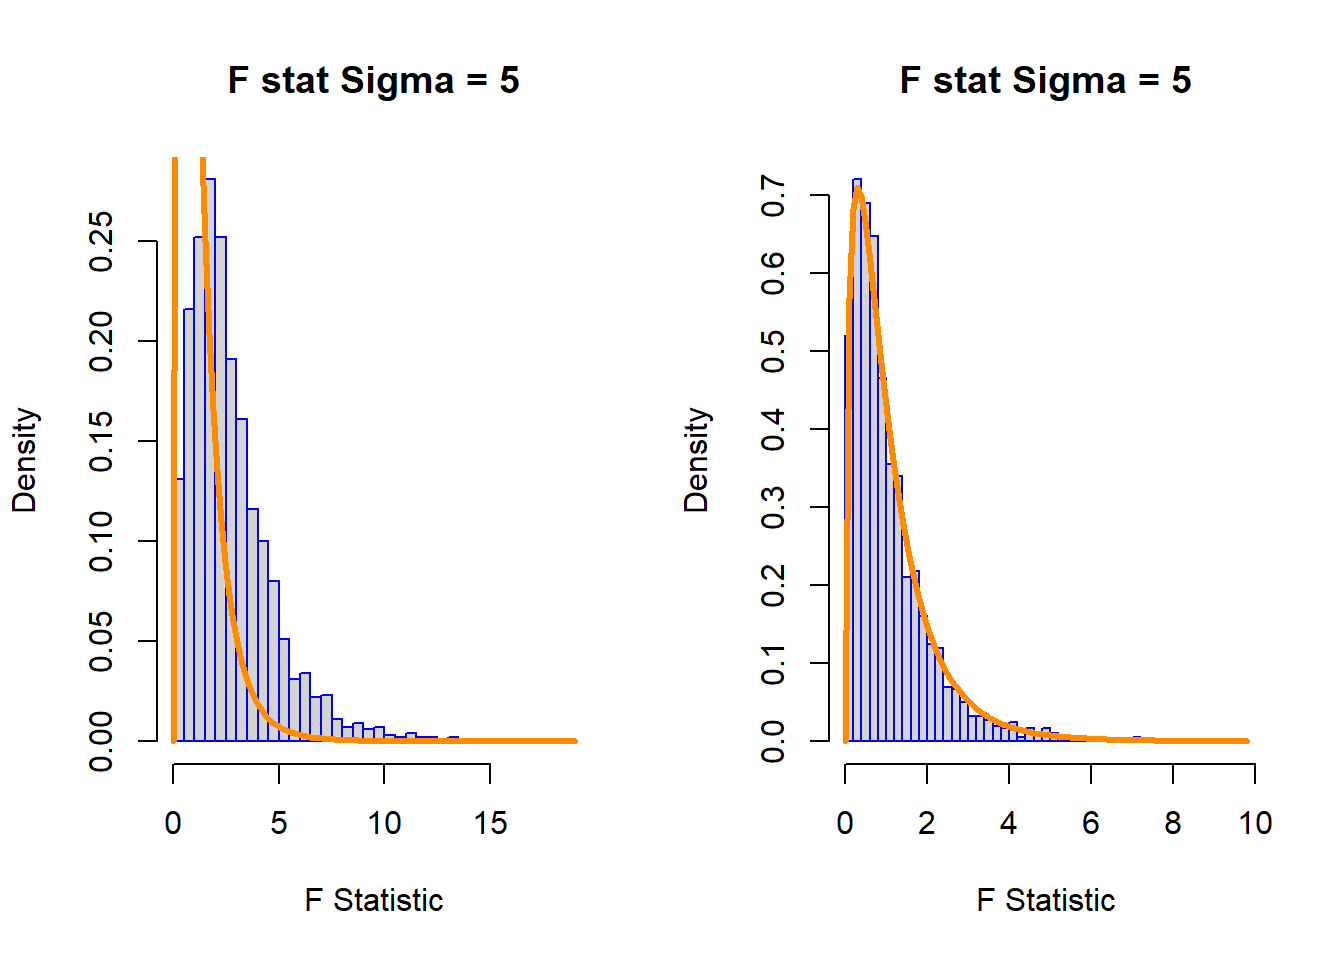
\includegraphics{FinalProject1.1_files/figure-latex/unnamed-chunk-5-1.pdf}

The distribution depicts that ``island'' has the least count and ``1H
OCEAN'' has the maximum count. This data also make practical sense.

\begin{Shaded}
\begin{Highlighting}[]
\KeywordTok{pairs}\NormalTok{(data, }\DataTypeTok{col =} \StringTok{"dodgerblue"}\NormalTok{)}
\end{Highlighting}
\end{Shaded}

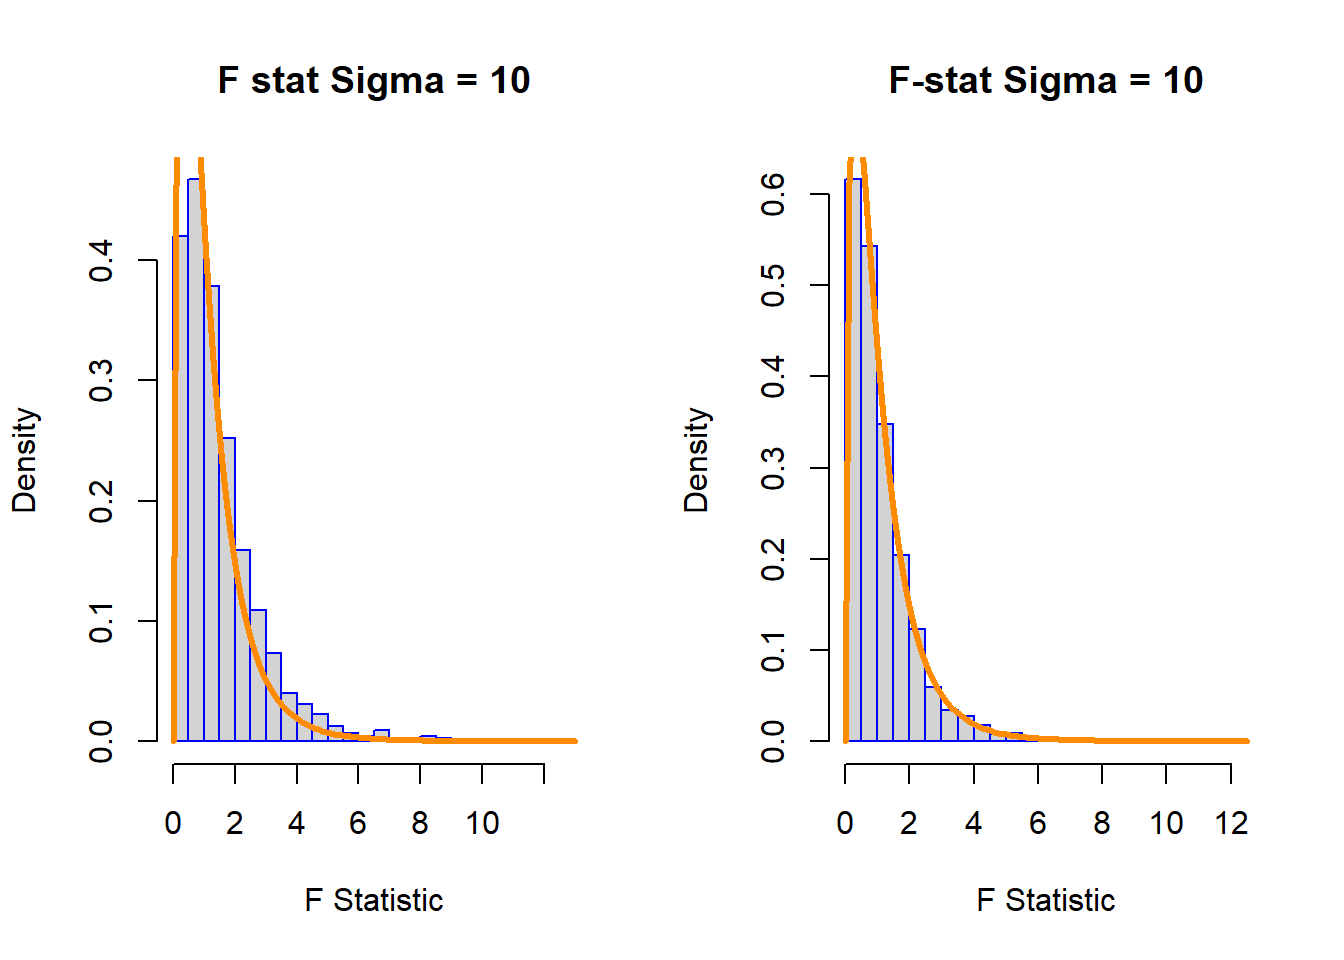
\includegraphics{FinalProject1.1_files/figure-latex/unnamed-chunk-6-1.pdf}

\begin{Shaded}
\begin{Highlighting}[]
\KeywordTok{kable}\NormalTok{(}\KeywordTok{t}\NormalTok{(}\KeywordTok{cor}\NormalTok{(data[,}\OperatorTok{-}\DecValTok{10}\NormalTok{])))}
\end{Highlighting}
\end{Shaded}

\begin{longtable}[]{@{}lrrrrrrrrr@{}}
\toprule
& longitude & latitude & housing\_median\_age & total\_rooms &
total\_bedrooms & population & households & median\_income &
median\_house\_value\tabularnewline
\midrule
\endhead
longitude & 1.0000000 & -0.9246161 & -0.1093565 & 0.0454802 & 0.0696080
& 0.1002703 & 0.0565128 & -0.0155502 & -0.0453982\tabularnewline
latitude & -0.9246161 & 1.0000000 & 0.0118991 & -0.0366668 & -0.0669828
& -0.1089973 & -0.0717742 & -0.0796263 & -0.1446382\tabularnewline
housing\_median\_age & -0.1093565 & 0.0118991 & 1.0000000 & -0.3606283 &
-0.3204510 & -0.2957873 & -0.3027680 & -0.1182777 &
0.1064320\tabularnewline
total\_rooms & 0.0454802 & -0.0366668 & -0.3606283 & 1.0000000 &
0.9303795 & 0.8572813 & 0.9189915 & 0.1978815 & 0.1332941\tabularnewline
total\_bedrooms & 0.0696080 & -0.0669828 & -0.3204510 & 0.9303795 &
1.0000000 & 0.8777467 & 0.9797283 & -0.0077228 &
0.0496862\tabularnewline
population & 0.1002703 & -0.1089973 & -0.2957873 & 0.8572813 & 0.8777467
& 1.0000000 & 0.9071859 & 0.0050866 & -0.0252997\tabularnewline
households & 0.0565128 & -0.0717742 & -0.3027680 & 0.9189915 & 0.9797283
& 0.9071859 & 1.0000000 & 0.0134339 & 0.0648935\tabularnewline
median\_income & -0.0155502 & -0.0796263 & -0.1182777 & 0.1978815 &
-0.0077228 & 0.0050866 & 0.0134339 & 1.0000000 &
0.6883555\tabularnewline
median\_house\_value & -0.0453982 & -0.1446382 & 0.1064320 & 0.1332941 &
0.0496862 & -0.0252997 & 0.0648935 & 0.6883555 &
1.0000000\tabularnewline
\bottomrule
\end{longtable}

\textbf{We noticed there is collinearity between {(households and
total\_bedrooms) \& (households and total\_rooms)}. We will keep this in
mind and explore the data further}

\hypertarget{training-and-test-data}{%
\subsubsection{Training and Test Data}\label{training-and-test-data}}

We took 80\% of the data as training data and used seed to be consistent
with the results.

\begin{Shaded}
\begin{Highlighting}[]
\KeywordTok{set.seed}\NormalTok{(}\DecValTok{100}\NormalTok{)}
\NormalTok{totalnrows =}\StringTok{ }\KeywordTok{nrow}\NormalTok{(data)}

\NormalTok{x =}\StringTok{ }\KeywordTok{sample}\NormalTok{(totalnrows, }\KeywordTok{floor}\NormalTok{(totalnrows }\OperatorTok{*}\StringTok{ }\FloatTok{.80}\NormalTok{) )}
\NormalTok{train_data =}\StringTok{ }\NormalTok{data[x, ]}
\NormalTok{test_data =}\StringTok{ }\NormalTok{data[}\OperatorTok{-}\NormalTok{x, ]}
\end{Highlighting}
\end{Shaded}

\begin{Shaded}
\begin{Highlighting}[]
\NormalTok{plot_map =}\StringTok{ }\KeywordTok{ggplot}\NormalTok{(train_data, }
                  \KeywordTok{aes}\NormalTok{(}\DataTypeTok{x =}\NormalTok{ longitude, }\DataTypeTok{y =}\NormalTok{ latitude, }\DataTypeTok{color =}\NormalTok{ median_house_value, }
                      \DataTypeTok{hma =}\NormalTok{ housing_median_age, }\DataTypeTok{tr =}\NormalTok{ total_rooms, }\DataTypeTok{tb =}\NormalTok{ total_bedrooms,}
                      \DataTypeTok{hh =}\NormalTok{ households, }\DataTypeTok{mi =}\NormalTok{ median_income)) }\OperatorTok{+}
\StringTok{              }\KeywordTok{geom_point}\NormalTok{(}\KeywordTok{aes}\NormalTok{(}\DataTypeTok{size =}\NormalTok{ population), }\DataTypeTok{alpha =} \FloatTok{0.4}\NormalTok{) }\OperatorTok{+}
\StringTok{              }\KeywordTok{xlab}\NormalTok{(}\StringTok{"Longitude"}\NormalTok{) }\OperatorTok{+}
\StringTok{              }\KeywordTok{ylab}\NormalTok{(}\StringTok{"Latitude"}\NormalTok{) }\OperatorTok{+}
\StringTok{              }\KeywordTok{ggtitle}\NormalTok{(}\StringTok{"Data Map - Longtitude vs Latitude and Associated Variables"}\NormalTok{) }\OperatorTok{+}
\StringTok{              }\KeywordTok{theme}\NormalTok{(}\DataTypeTok{plot.title =} \KeywordTok{element_text}\NormalTok{(}\DataTypeTok{hjust =} \FloatTok{0.5}\NormalTok{)) }\OperatorTok{+}
\StringTok{              }\KeywordTok{scale_color_distiller}\NormalTok{(}\DataTypeTok{palette =} \StringTok{"Paired"}\NormalTok{, }\DataTypeTok{labels =}\NormalTok{ comma) }\OperatorTok{+}
\StringTok{              }\KeywordTok{labs}\NormalTok{(}\DataTypeTok{color =} \StringTok{"Median House Value (in $USD)"}\NormalTok{, }\DataTypeTok{size =} \StringTok{"Population"}\NormalTok{)}
\NormalTok{plot_map}
\end{Highlighting}
\end{Shaded}

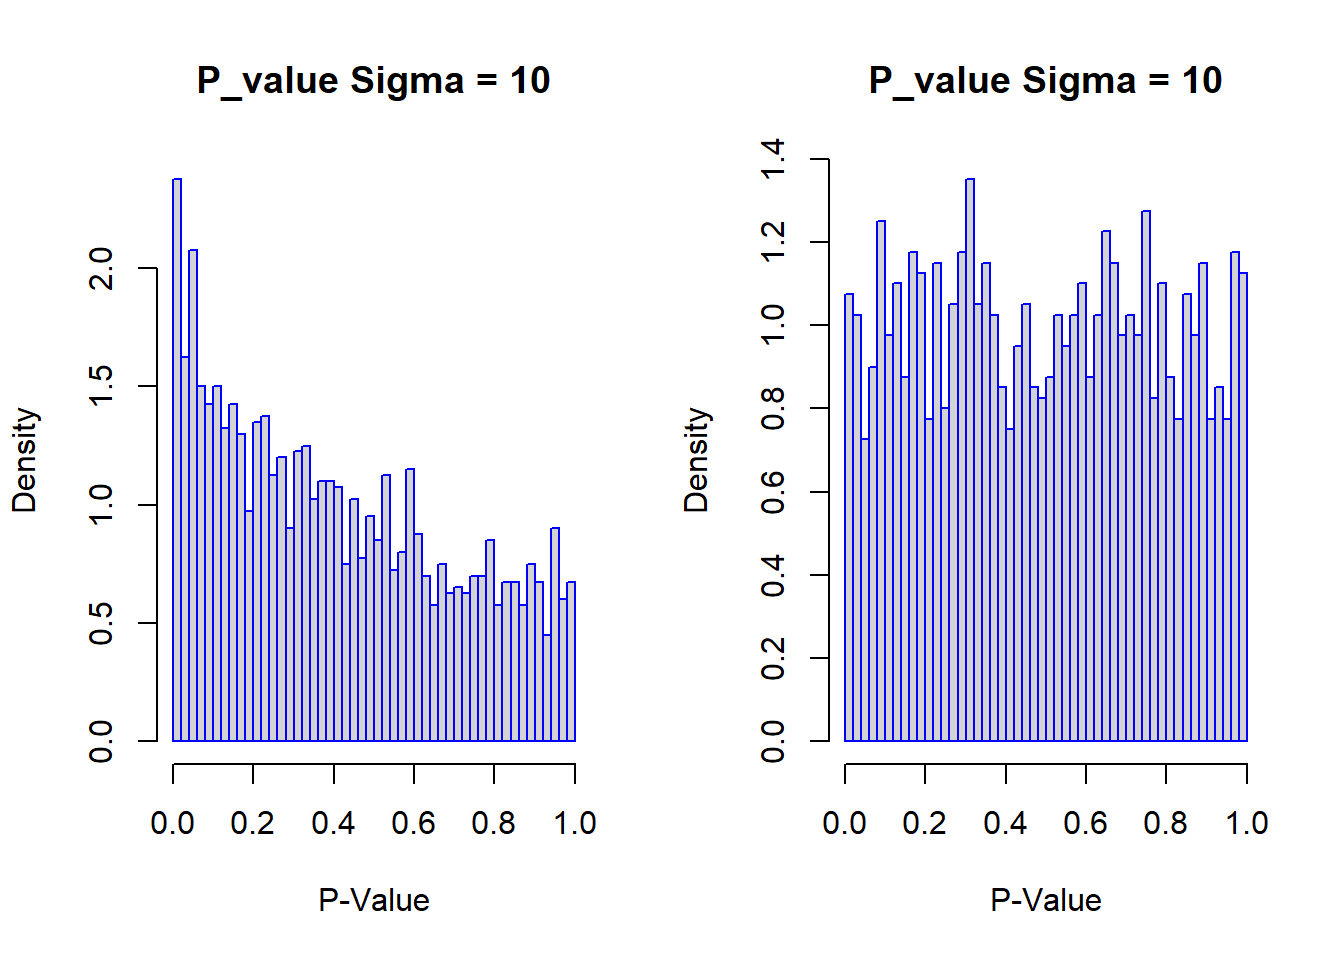
\includegraphics{FinalProject1.1_files/figure-latex/unnamed-chunk-9-1.pdf}

The graph above shows distribution of Median house value based on
population and Latitude. It gives us fair distribution of values across
geographical area.

{Additive Model}

\begin{Shaded}
\begin{Highlighting}[]
\CommentTok{#Training additive Model}
\NormalTok{model_add =}\StringTok{ }\KeywordTok{lm}\NormalTok{(median_house_value }\OperatorTok{~}\StringTok{ }\NormalTok{., }\DataTypeTok{data =}\NormalTok{ train_data)}
\KeywordTok{summary}\NormalTok{(model_add)}
\end{Highlighting}
\end{Shaded}

\begin{verbatim}
## 
## Call:
## lm(formula = median_house_value ~ ., data = train_data)
## 
## Residuals:
##     Min      1Q  Median      3Q     Max 
## -554770  -42731  -10480   28801  761094 
## 
## Coefficients:
##                             Estimate Std. Error t value Pr(>|t|)    
## (Intercept)               -2.274e+06  9.846e+04 -23.096  < 2e-16 ***
## longitude                 -2.681e+04  1.140e+03 -23.512  < 2e-16 ***
## latitude                  -2.540e+04  1.123e+03 -22.609  < 2e-16 ***
## housing_median_age         1.102e+03  4.885e+01  22.557  < 2e-16 ***
## total_rooms               -5.850e+00  8.771e-01  -6.670 2.64e-11 ***
## total_bedrooms             9.931e+01  7.737e+00  12.835  < 2e-16 ***
## population                -3.732e+01  1.183e+00 -31.533  < 2e-16 ***
## households                 4.817e+01  8.405e+00   5.731 1.02e-08 ***
## median_income              3.905e+04  3.740e+02 104.386  < 2e-16 ***
## ocean_proximityINLAND     -3.966e+04  1.954e+03 -20.295  < 2e-16 ***
## ocean_proximityISLAND      1.531e+05  3.068e+04   4.990 6.09e-07 ***
## ocean_proximityNEAR BAY   -4.041e+03  2.122e+03  -1.904  0.05691 .  
## ocean_proximityNEAR OCEAN  5.578e+03  1.744e+03   3.199  0.00138 ** 
## ---
## Signif. codes:  0 '***' 0.001 '**' 0.01 '*' 0.05 '.' 0.1 ' ' 1
## 
## Residual standard error: 68490 on 16333 degrees of freedom
## Multiple R-squared:  0.6471, Adjusted R-squared:  0.6469 
## F-statistic:  2496 on 12 and 16333 DF,  p-value: < 2.2e-16
\end{verbatim}

\begin{Shaded}
\begin{Highlighting}[]
\KeywordTok{summary}\NormalTok{(model_add)}\OperatorTok{$}\NormalTok{adj.r.squared}
\end{Highlighting}
\end{Shaded}

\begin{verbatim}
## [1] 0.6468567
\end{verbatim}

\textbf{By analyzing p-value of all Beta variable in Additive model, we
can say that we fail to reject that Null Hypothesis that Beta value of
any variable is Zero. Hence all variables are playing important role in
prediction of House Median Income. And Adjusted R squared value of Model
is 64.6\%}

{Interaction Model}

\begin{Shaded}
\begin{Highlighting}[]
\NormalTok{model_int =}\StringTok{ }\KeywordTok{lm}\NormalTok{(median_house_value }\OperatorTok{~}\StringTok{ }\NormalTok{. }\OperatorTok{^}\StringTok{ }\DecValTok{2}\NormalTok{, }\DataTypeTok{data =}\NormalTok{ train_data)}
\KeywordTok{summary}\NormalTok{(model_int)}\OperatorTok{$}\NormalTok{adj.r.squared}
\end{Highlighting}
\end{Shaded}

\begin{verbatim}
## [1] 0.7025208
\end{verbatim}

\textbf{In interaction model we can see an increment of Model
performance by Adjusted R Squared which is 70.3\%}

{ Testing Interaction model with respect to Additive Model}

\begin{Shaded}
\begin{Highlighting}[]
\KeywordTok{anova}\NormalTok{(model_int, model_add)}
\end{Highlighting}
\end{Shaded}

\begin{verbatim}
## Analysis of Variance Table
## 
## Model 1: median_house_value ~ (longitude + latitude + housing_median_age + 
##     total_rooms + total_bedrooms + population + households + 
##     median_income + ocean_proximity)^2
## Model 2: median_house_value ~ longitude + latitude + housing_median_age + 
##     total_rooms + total_bedrooms + population + households + 
##     median_income + ocean_proximity
##   Res.Df        RSS  Df   Sum of Sq      F    Pr(>F)    
## 1  16277 6.4322e+13                                     
## 2  16333 7.6621e+13 -56 -1.2299e+13 55.575 < 2.2e-16 ***
## ---
## Signif. codes:  0 '***' 0.001 '**' 0.01 '*' 0.05 '.' 0.1 ' ' 1
\end{verbatim}

\textbf{P-value of test is 2.2e-16 which is very less hence we can
consider Interactive models is better than additive model}

\hypertarget{model-improvement-using-aic-and-bic}{%
\subsubsection{Model Improvement Using AIC and
BIC}\label{model-improvement-using-aic-and-bic}}

\begin{Shaded}
\begin{Highlighting}[]
\NormalTok{model_add_aic =}\StringTok{ }\KeywordTok{step}\NormalTok{(model_add, }\DataTypeTok{direction =} \StringTok{"backward"}\NormalTok{, }\DataTypeTok{trace =} \DecValTok{0}\NormalTok{)}
\KeywordTok{summary}\NormalTok{(model_add_aic)}\OperatorTok{$}\NormalTok{adj.r.squared}
\end{Highlighting}
\end{Shaded}

\begin{verbatim}
## [1] 0.6468567
\end{verbatim}

\begin{Shaded}
\begin{Highlighting}[]
\NormalTok{model_add_bic =}\StringTok{ }\KeywordTok{step}\NormalTok{(model_add, }\DataTypeTok{direction =} \StringTok{"backward"}\NormalTok{, }\DataTypeTok{trace =} \DecValTok{0}\NormalTok{, }\DataTypeTok{k =} \KeywordTok{log}\NormalTok{(}\KeywordTok{nrow}\NormalTok{(train_data)))}
\KeywordTok{summary}\NormalTok{(model_add_bic)}\OperatorTok{$}\NormalTok{adj.r.squared}
\end{Highlighting}
\end{Shaded}

\begin{verbatim}
## [1] 0.6468567
\end{verbatim}

\begin{Shaded}
\begin{Highlighting}[]
\NormalTok{model_int_aic =}\StringTok{ }\KeywordTok{step}\NormalTok{(model_int, }\DataTypeTok{direction =} \StringTok{"backward"}\NormalTok{, }\DataTypeTok{trace =} \DecValTok{0}\NormalTok{)}
\KeywordTok{summary}\NormalTok{(model_int_aic)}\OperatorTok{$}\NormalTok{adj.r.squared}
\end{Highlighting}
\end{Shaded}

\begin{verbatim}
## [1] 0.7025212
\end{verbatim}

\begin{Shaded}
\begin{Highlighting}[]
\NormalTok{model_int_bic =}\StringTok{ }\KeywordTok{step}\NormalTok{(model_int, }\DataTypeTok{direction =} \StringTok{"backward"}\NormalTok{, }\DataTypeTok{trace =} \DecValTok{0}\NormalTok{, }\DataTypeTok{k =} \KeywordTok{log}\NormalTok{(}\KeywordTok{nrow}\NormalTok{(train_data)))}
\KeywordTok{summary}\NormalTok{(model_int_bic)}\OperatorTok{$}\NormalTok{adj.r.squared}
\end{Highlighting}
\end{Shaded}

\begin{verbatim}
## [1] 0.7019587
\end{verbatim}

\begin{Shaded}
\begin{Highlighting}[]
\NormalTok{beginning_mods_results =}\StringTok{ }\KeywordTok{data.frame}\NormalTok{(}
  \StringTok{"Total Predictors"}\NormalTok{ =}
\StringTok{    }\KeywordTok{c}\NormalTok{(}\StringTok{"Additive Model"}\NormalTok{ =}\StringTok{ }\KeywordTok{extractAIC}\NormalTok{(model_add)[}\DecValTok{1}\NormalTok{],}
      \StringTok{"Interaction Model"}\NormalTok{ =}\StringTok{ }\KeywordTok{extractAIC}\NormalTok{(model_int)[}\DecValTok{1}\NormalTok{],}
      \StringTok{"AIC_additive Model"}\NormalTok{ =}\StringTok{ }\KeywordTok{extractAIC}\NormalTok{(model_add_aic)[}\DecValTok{1}\NormalTok{],}
      \StringTok{"AIC_Int Model"}\NormalTok{ =}\StringTok{ }\KeywordTok{extractAIC}\NormalTok{(model_int_aic)[}\DecValTok{1}\NormalTok{],}
      \StringTok{"BIC_additive Model"}\NormalTok{ =}\StringTok{ }\KeywordTok{extractAIC}\NormalTok{(model_add_bic)[}\DecValTok{1}\NormalTok{],}
      \StringTok{"BIC_Int Model"}\NormalTok{ =}\StringTok{ }\KeywordTok{extractAIC}\NormalTok{(model_int_bic)[}\DecValTok{1}\NormalTok{]),}
  \StringTok{"AIC"}\NormalTok{ =}
\StringTok{    }\KeywordTok{c}\NormalTok{(}\StringTok{"Additive Model"}\NormalTok{ =}\StringTok{ }\KeywordTok{extractAIC}\NormalTok{(model_add)[}\DecValTok{2}\NormalTok{],}
       \StringTok{"Interaction Model"}\NormalTok{ =}\StringTok{ }\KeywordTok{extractAIC}\NormalTok{(model_int)[}\DecValTok{2}\NormalTok{],}
      \StringTok{"AIC_additive Model"}\NormalTok{ =}\StringTok{ }\KeywordTok{extractAIC}\NormalTok{(model_add_aic)[}\DecValTok{2}\NormalTok{],}
      \StringTok{"AIC_Int Model"}\NormalTok{ =}\StringTok{ }\KeywordTok{extractAIC}\NormalTok{(model_int_aic)[}\DecValTok{2}\NormalTok{],}
       \StringTok{"BIC_additive Model"}\NormalTok{ =}\StringTok{ }\KeywordTok{extractAIC}\NormalTok{(model_add_bic)[}\DecValTok{2}\NormalTok{],}
      \StringTok{"BIC_Int Model"}\NormalTok{ =}\StringTok{ }\KeywordTok{extractAIC}\NormalTok{(model_int_bic)[}\DecValTok{2}\NormalTok{]),}
  \StringTok{"Adj R-Squared"}\NormalTok{ =}
\StringTok{    }\KeywordTok{c}\NormalTok{(}\StringTok{"Additive Model"}\NormalTok{ =}\StringTok{ }\KeywordTok{summary}\NormalTok{(model_add)}\OperatorTok{$}\NormalTok{adj.r.squared,}
      \StringTok{"Interaction Model"}\NormalTok{ =}\StringTok{ }\KeywordTok{summary}\NormalTok{(model_int)}\OperatorTok{$}\NormalTok{adj.r.squared,}
      \StringTok{"AIC_additive Model"}\NormalTok{ =}\KeywordTok{summary}\NormalTok{(model_add_aic)}\OperatorTok{$}\NormalTok{adj.r.squared,}
      \StringTok{"AIC_Int Model"}\NormalTok{ =}\StringTok{ }\KeywordTok{summary}\NormalTok{(model_int_aic)}\OperatorTok{$}\NormalTok{adj.r.squared,}
       \StringTok{"BIC_additive Model"}\NormalTok{ =}\KeywordTok{summary}\NormalTok{((model_add_bic))}\OperatorTok{$}\NormalTok{adj.r.squared,}
      \StringTok{"BIC_Int Model"}\NormalTok{ =}\StringTok{ }\KeywordTok{summary}\NormalTok{(model_int_bic)}\OperatorTok{$}\NormalTok{adj.r.squared))}

\KeywordTok{kable}\NormalTok{(beginning_mods_results, }\DataTypeTok{align =} \KeywordTok{c}\NormalTok{(}\StringTok{"c"}\NormalTok{, }\StringTok{"r"}\NormalTok{))}
\end{Highlighting}
\end{Shaded}

\begin{longtable}[]{@{}lcrc@{}}
\toprule
& Total.Predictors & AIC & Adj.R.Squared\tabularnewline
\midrule
\endhead
Additive Model & 13 & 364021.2 & 0.6468567\tabularnewline
Interaction Model & 69 & 361273.2 & 0.7025208\tabularnewline
AIC\_additive Model & 13 & 364021.2 & 0.6468567\tabularnewline
AIC\_Int Model & 64 & 361268.2 & 0.7025212\tabularnewline
BIC\_additive Model & 13 & 364021.2 & 0.6468567\tabularnewline
BIC\_Int Model & 56 & 361291.2 & 0.7019587\tabularnewline
\bottomrule
\end{longtable}

\textbf{We see that the model with the best (i.e., lowest) AIC is
Interaction Model, with a score of 361268.2. But we will work further to
enhance performance of model.}

\begin{Shaded}
\begin{Highlighting}[]
\NormalTok{diagnostics =}\StringTok{ }\ControlFlowTok{function}\NormalTok{(model, }\DataTypeTok{alpha =} \FloatTok{.05}\NormalTok{, }\DataTypeTok{pointcol =} \StringTok{"orange"}\NormalTok{, }\DataTypeTok{linecol =} \StringTok{"blue"}\NormalTok{, }\DataTypeTok{plots =} \OtherTok{TRUE}\NormalTok{, }\DataTypeTok{tests =} \OtherTok{TRUE}\NormalTok{, }\DataTypeTok{pointtype =} \DecValTok{16}\NormalTok{) \{}
    \ControlFlowTok{if}\NormalTok{ (plots }\OperatorTok{==}\StringTok{ }\OtherTok{TRUE}\NormalTok{) \{}
        \KeywordTok{par}\NormalTok{(}\DataTypeTok{mfrow =} \KeywordTok{c}\NormalTok{(}\DecValTok{1}\NormalTok{, }\DecValTok{3}\NormalTok{))}
        \KeywordTok{plot}\NormalTok{(}
                \KeywordTok{fitted}\NormalTok{(model),}
                \KeywordTok{resid}\NormalTok{(model),}
                \DataTypeTok{pch =}\NormalTok{ pointtype,}
                \DataTypeTok{xlab =} \StringTok{"Fitted Values"}\NormalTok{,}
                \DataTypeTok{ylab =} \StringTok{"Residuals"}\NormalTok{,}
                \DataTypeTok{main =} \StringTok{"Fitted vs Residuals"}\NormalTok{,}
                \DataTypeTok{col =}\NormalTok{ pointcol}
\NormalTok{            )}
        \KeywordTok{abline}\NormalTok{(}\DataTypeTok{h =} \DecValTok{0}\NormalTok{, }\DataTypeTok{lwd =} \DecValTok{2}\NormalTok{, }\DataTypeTok{col =}\NormalTok{ linecol)}
        
        \KeywordTok{qqnorm}\NormalTok{(}
                \KeywordTok{resid}\NormalTok{(model),}
                \DataTypeTok{pch =}\NormalTok{ pointtype,}
                \DataTypeTok{main =} \StringTok{"QQNorm Plot"}\NormalTok{,}
                \DataTypeTok{col =}\NormalTok{ pointcol}
\NormalTok{            )}
        \KeywordTok{qqline}\NormalTok{(}
                \KeywordTok{resid}\NormalTok{(model),}
                \DataTypeTok{lwd =} \DecValTok{2}\NormalTok{,}
                \DataTypeTok{col =}\NormalTok{ linecol}
\NormalTok{                )}
        \KeywordTok{hist}\NormalTok{(}
            \KeywordTok{resid}\NormalTok{(model),}
            \DataTypeTok{main =} \StringTok{"Histogram of Residuals"}\NormalTok{,}
            \DataTypeTok{col =}\NormalTok{ pointcol,}
            \DataTypeTok{xlab =} \StringTok{"Residuals"}\NormalTok{,}
            \DataTypeTok{ylab =} \StringTok{"Frequency"}
\NormalTok{            )}
\NormalTok{    \}}
    \ControlFlowTok{if}\NormalTok{ (tests }\OperatorTok{==}\StringTok{ }\OtherTok{TRUE}\NormalTok{) \{}
\NormalTok{        ks_test =}\StringTok{ }\KeywordTok{ks.test}\NormalTok{(}\KeywordTok{resid}\NormalTok{(model),}\DataTypeTok{y=}\StringTok{'pnorm'}\NormalTok{,}\DataTypeTok{alternative=}\StringTok{'two.sided'}\NormalTok{)}
\NormalTok{        bp_test =}\StringTok{ }\KeywordTok{bptest}\NormalTok{(model)}
\NormalTok{        test_results =}\StringTok{ }\KeywordTok{data.frame}\NormalTok{(}
          \StringTok{"Kolmogorov-Smirnov  Test"}\NormalTok{ =}
\StringTok{            }\KeywordTok{c}\NormalTok{(}\StringTok{"Test Statistic"}\NormalTok{ =}\StringTok{ }\KeywordTok{round}\NormalTok{(ks_test}\OperatorTok{$}\NormalTok{statistic, }\DecValTok{5}\NormalTok{),}
              \StringTok{"P-Value"}\NormalTok{ =}\StringTok{ }\NormalTok{ks_test}\OperatorTok{$}\NormalTok{p.value,}
              \StringTok{"Result"}\NormalTok{ =}\StringTok{ }\KeywordTok{ifelse}\NormalTok{(ks_test}\OperatorTok{$}\NormalTok{p.value }\OperatorTok{<}\StringTok{ }\NormalTok{alpha, }\StringTok{"Reject"}\NormalTok{, }\StringTok{"Fail To Reject"}\NormalTok{)),}
          \StringTok{"Breusch-Pagan Test"}\NormalTok{ =}
\StringTok{            }\KeywordTok{c}\NormalTok{(}\StringTok{"Test Statistic"}\NormalTok{ =}\StringTok{ }\KeywordTok{round}\NormalTok{(bp_test}\OperatorTok{$}\NormalTok{statistic, }\DecValTok{5}\NormalTok{),}
              \StringTok{"P-Value"}\NormalTok{ =}\StringTok{ }\NormalTok{bp_test}\OperatorTok{$}\NormalTok{p.value,}
              \StringTok{"Result"}\NormalTok{ =}\StringTok{ }\KeywordTok{ifelse}\NormalTok{(bp_test}\OperatorTok{$}\NormalTok{p.value }\OperatorTok{<}\StringTok{ }\NormalTok{alpha, }\StringTok{"Reject"}\NormalTok{, }\StringTok{"Fail To Reject"}\NormalTok{)))}

        \KeywordTok{kable}\NormalTok{(}\KeywordTok{t}\NormalTok{(test_results), }\DataTypeTok{col.names =} \KeywordTok{c}\NormalTok{(}\StringTok{"Test Statistic"}\NormalTok{, }\StringTok{"P-Value"}\NormalTok{, }\StringTok{"Decision"}\NormalTok{))}
\NormalTok{    \}}
\NormalTok{\}}
\end{Highlighting}
\end{Shaded}

\begin{Shaded}
\begin{Highlighting}[]
\KeywordTok{diagnostics}\NormalTok{(model_add)}
\end{Highlighting}
\end{Shaded}

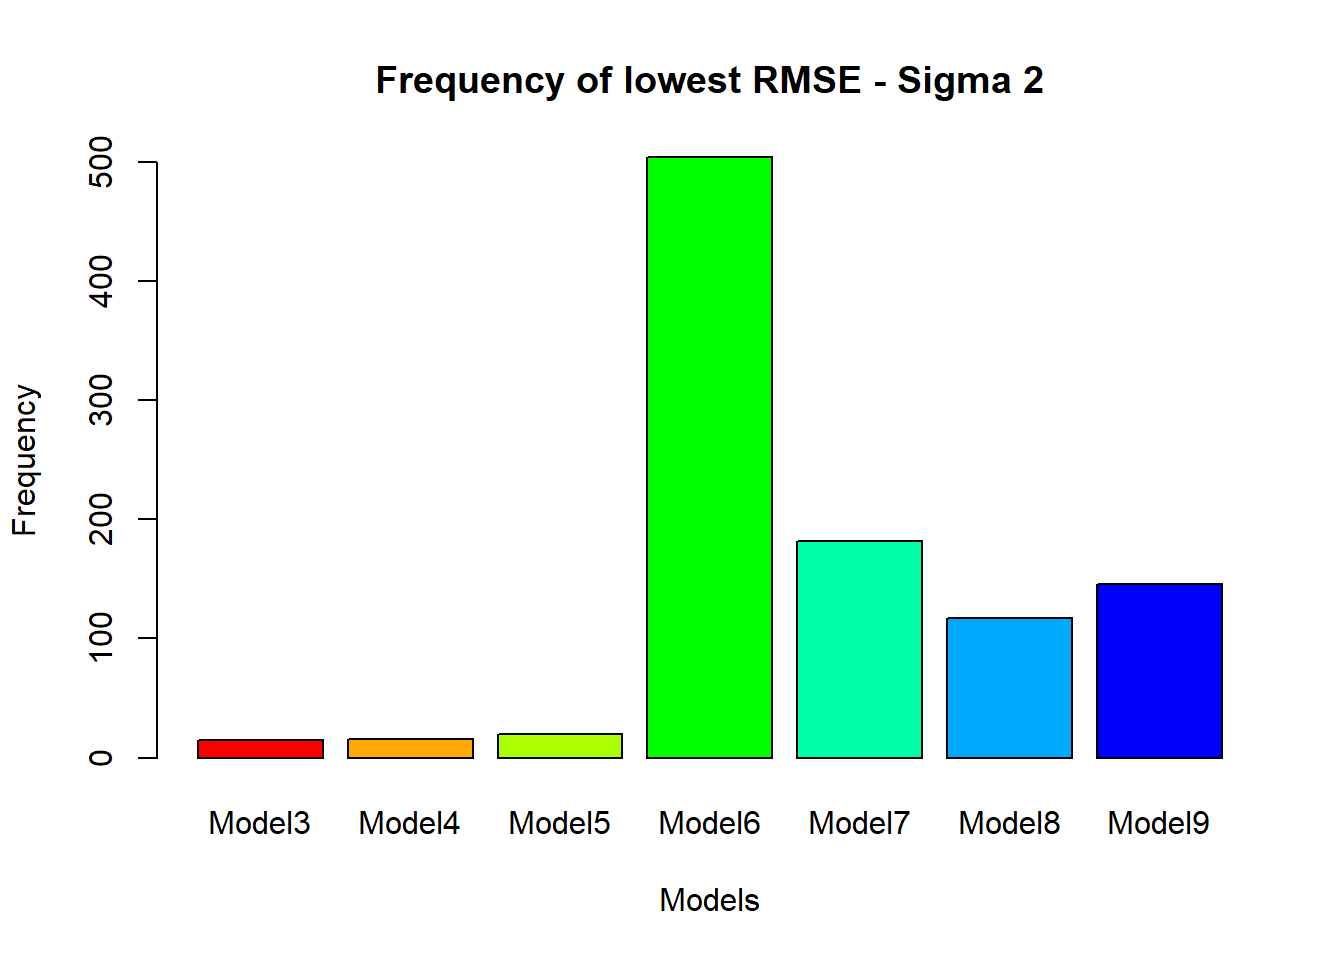
\includegraphics{FinalProject1.1_files/figure-latex/unnamed-chunk-16-1.pdf}

\begin{longtable}[]{@{}llll@{}}
\toprule
& Test Statistic & P-Value & Decision\tabularnewline
\midrule
\endhead
Kolmogorov.Smirnov..Test & 0.5802 & 0 & Reject\tabularnewline
Breusch.Pagan.Test & 813.50284 & 2.10341410745741e-166 &
Reject\tabularnewline
\bottomrule
\end{longtable}

\begin{Shaded}
\begin{Highlighting}[]
\KeywordTok{diagnostics}\NormalTok{(model_int)}
\end{Highlighting}
\end{Shaded}

\includegraphics{FinalProject1.1_files/figure-latex/unnamed-chunk-16-2.pdf}

\begin{longtable}[]{@{}llll@{}}
\toprule
& Test Statistic & P-Value & Decision\tabularnewline
\midrule
\endhead
Kolmogorov.Smirnov..Test & 0.57806 & 0 & Reject\tabularnewline
Breusch.Pagan.Test & 1698.68853 & 7.46002686123318e-310 &
Reject\tabularnewline
\bottomrule
\end{longtable}

\begin{Shaded}
\begin{Highlighting}[]
\KeywordTok{diagnostics}\NormalTok{(model_add_aic)}
\end{Highlighting}
\end{Shaded}

\begin{longtable}[]{@{}llll@{}}
\toprule
& Test Statistic & P-Value & Decision\tabularnewline
\midrule
\endhead
Kolmogorov.Smirnov..Test & 0.5802 & 0 & Reject\tabularnewline
Breusch.Pagan.Test & 813.50284 & 2.10341410745741e-166 &
Reject\tabularnewline
\bottomrule
\end{longtable}

\begin{Shaded}
\begin{Highlighting}[]
\KeywordTok{diagnostics}\NormalTok{(model_add_bic)}
\end{Highlighting}
\end{Shaded}

\includegraphics{FinalProject1.1_files/figure-latex/unnamed-chunk-16-3.pdf}

\begin{longtable}[]{@{}llll@{}}
\toprule
& Test Statistic & P-Value & Decision\tabularnewline
\midrule
\endhead
Kolmogorov.Smirnov..Test & 0.5802 & 0 & Reject\tabularnewline
Breusch.Pagan.Test & 813.50284 & 2.10341410745741e-166 &
Reject\tabularnewline
\bottomrule
\end{longtable}

\begin{Shaded}
\begin{Highlighting}[]
\KeywordTok{diagnostics}\NormalTok{(model_int_aic)}
\end{Highlighting}
\end{Shaded}

\includegraphics{FinalProject1.1_files/figure-latex/unnamed-chunk-16-4.pdf}

\begin{longtable}[]{@{}llll@{}}
\toprule
& Test Statistic & P-Value & Decision\tabularnewline
\midrule
\endhead
Kolmogorov.Smirnov..Test & 0.57873 & 0 & Reject\tabularnewline
Breusch.Pagan.Test & 1589.03891 & 1.76669099023126e-290 &
Reject\tabularnewline
\bottomrule
\end{longtable}

\begin{Shaded}
\begin{Highlighting}[]
\KeywordTok{diagnostics}\NormalTok{(model_int_bic)}
\end{Highlighting}
\end{Shaded}

\includegraphics{FinalProject1.1_files/figure-latex/unnamed-chunk-16-5.pdf}

\begin{longtable}[]{@{}llll@{}}
\toprule
& Test Statistic & P-Value & Decision\tabularnewline
\midrule
\endhead
Kolmogorov.Smirnov..Test & 0.57776 & 0 & Reject\tabularnewline
Breusch.Pagan.Test & 1436.29723 & 3.15291874921026e-264 &
Reject\tabularnewline
\bottomrule
\end{longtable}

\begin{Shaded}
\begin{Highlighting}[]
\NormalTok{x =}\StringTok{ }\KeywordTok{ks.test}\NormalTok{(}\DataTypeTok{x=}\KeywordTok{rnorm}\NormalTok{(}\DecValTok{10}\OperatorTok{^}\DecValTok{4}\NormalTok{),}\DataTypeTok{y=}\StringTok{'pnorm'}\NormalTok{,}\DataTypeTok{alternative=}\StringTok{'two.sided'}\NormalTok{)}

\NormalTok{x}\OperatorTok{$}\NormalTok{p.value}
\end{Highlighting}
\end{Shaded}

\begin{verbatim}
## [1] 0.9685713
\end{verbatim}

We can see that all above models do not have Equal variance and residual
in Normal form. Hence we need to improve model.

Kolmogorov--Smirnov test- In statistics, the Kolmogorov--Smirnov test is
a nonparametric test of the equality of continuous, one-dimensional
probability distributions that can be used to compare a sample with a
reference probability distribution, or to compare two samples. Note- We
tried using shapiro.test first, but the test that did not work
considering the size of the dataset.

\hypertarget{model-improvement}{%
\subsubsection{Model Improvement}\label{model-improvement}}

Now, we will calculate the cooks distance and will remove outliers and
high influential values.

\begin{Shaded}
\begin{Highlighting}[]
\NormalTok{value =}\StringTok{ }\KeywordTok{cooks.distance}\NormalTok{(model_add)}
\KeywordTok{sum}\NormalTok{(value }\OperatorTok{>}\StringTok{ }\DecValTok{4} \OperatorTok{/}\StringTok{ }\KeywordTok{length}\NormalTok{(}\KeywordTok{resid}\NormalTok{(model_add)))}
\end{Highlighting}
\end{Shaded}

\begin{verbatim}
## [1] 885
\end{verbatim}

\begin{Shaded}
\begin{Highlighting}[]
\NormalTok{model_new_add =}\StringTok{  }\KeywordTok{lm}\NormalTok{(median_house_value }\OperatorTok{~}\StringTok{ }\NormalTok{., }\DataTypeTok{data =}\NormalTok{ train_data, }\DataTypeTok{subset =}\NormalTok{ value }\OperatorTok{<=}\StringTok{ }\NormalTok{(}\DecValTok{4} \OperatorTok{/}\StringTok{ }\KeywordTok{nrow}\NormalTok{(train_data)))}

\NormalTok{model_new_int =}\StringTok{  }\KeywordTok{lm}\NormalTok{(median_house_value }\OperatorTok{~}\StringTok{ }\NormalTok{.}\OperatorTok{^}\DecValTok{2}\NormalTok{, }\DataTypeTok{data =}\NormalTok{ train_data, }\DataTypeTok{subset =}\NormalTok{ value }\OperatorTok{<=}\StringTok{ }\NormalTok{(}\DecValTok{4} \OperatorTok{/}\StringTok{ }\KeywordTok{nrow}\NormalTok{(train_data)))}

\NormalTok{model_new_add_AIC =}\StringTok{ }\KeywordTok{step}\NormalTok{(model_new_add, }\DataTypeTok{direction =} \StringTok{"backward"}\NormalTok{, }\DataTypeTok{trace =} \DecValTok{0}\NormalTok{)}

\NormalTok{model_new_int_AIC =}\StringTok{ }\KeywordTok{step}\NormalTok{(model_new_int, }\DataTypeTok{direction =} \StringTok{"backward"}\NormalTok{, }\DataTypeTok{trace =} \DecValTok{0}\NormalTok{)}
\end{Highlighting}
\end{Shaded}

Based on the new data data values, we will again train the models and
calculate ADJ R Squared and LOOCV values (Leave-One-Out
Cross-Validation)

\hypertarget{results}{%
\subsection{Results}\label{results}}

When we initially calculated the AdjustedR2 value the results were not
very convincing as we had low ADJ R Squared value for all the models.
However,when we remove the outliers and high influential values using
the cooks distance we got better results.

\begin{Shaded}
\begin{Highlighting}[]
\NormalTok{Result =}\StringTok{ }\KeywordTok{data.frame}\NormalTok{(}
        \StringTok{"Additive Model"}\NormalTok{ =}\KeywordTok{c}\NormalTok{(}\StringTok{"LOOCV"}\NormalTok{ =}\StringTok{ }\KeywordTok{sqrt}\NormalTok{(}\KeywordTok{mean}\NormalTok{((}\KeywordTok{resid}\NormalTok{(model_new_add) }\OperatorTok{/}\StringTok{ }\NormalTok{(}\DecValTok{1} \OperatorTok{-}\StringTok{ }\KeywordTok{hatvalues}\NormalTok{(model_new_add))) }\OperatorTok{^}\StringTok{ }\DecValTok{2}\NormalTok{)),}
              \StringTok{"ADJ R Squared"}\NormalTok{ =}\StringTok{ }\KeywordTok{summary}\NormalTok{(model_new_add)}\OperatorTok{$}\NormalTok{adj.r.squared,}
              \StringTok{"Test RMSE"}\NormalTok{ =}\StringTok{ }\KeywordTok{sqrt}\NormalTok{(}\KeywordTok{mean}\NormalTok{((test_data}\OperatorTok{$}\NormalTok{median_house_value }\OperatorTok{-}\StringTok{ }\KeywordTok{predict}\NormalTok{(model_new_add, }\DataTypeTok{newdata =}\NormalTok{ test_data))}\OperatorTok{^}\DecValTok{2}\NormalTok{)),}
               \StringTok{"SE"}\NormalTok{ =}\StringTok{ }\KeywordTok{summary}\NormalTok{(model_new_add)}\OperatorTok{$}\NormalTok{sigma),}
        
        \StringTok{"Interaction Model"}\NormalTok{ =}\StringTok{ }\KeywordTok{c}\NormalTok{( }\StringTok{"LOOCV"}\NormalTok{ =}\StringTok{ }\KeywordTok{sqrt}\NormalTok{(}\KeywordTok{mean}\NormalTok{((}\KeywordTok{resid}\NormalTok{(model_new_int) }\OperatorTok{/}\StringTok{ }\NormalTok{(}\DecValTok{1} \OperatorTok{-}\StringTok{ }\KeywordTok{hatvalues}\NormalTok{(model_new_int))) }\OperatorTok{^}\StringTok{ }\DecValTok{2}\NormalTok{)),}
              \StringTok{"ADJ R Squared"}\NormalTok{ =}\StringTok{ }\KeywordTok{summary}\NormalTok{(model_new_int)}\OperatorTok{$}\NormalTok{adj.r.squared,}
              \StringTok{"Test RMSE"}\NormalTok{ =}\StringTok{ }\KeywordTok{sqrt}\NormalTok{(}\KeywordTok{mean}\NormalTok{((test_data}\OperatorTok{$}\NormalTok{median_house_value }\OperatorTok{-}\StringTok{ }\KeywordTok{predict}\NormalTok{(model_new_int, }\DataTypeTok{newdata =}\NormalTok{ test_data))}\OperatorTok{^}\DecValTok{2}\NormalTok{)),}
              \StringTok{"SE"}\NormalTok{ =}\StringTok{ }\KeywordTok{summary}\NormalTok{(model_new_int)}\OperatorTok{$}\NormalTok{sigma),}
        
        \StringTok{"Additive Model AIC"}\NormalTok{ =}\StringTok{ }\KeywordTok{c}\NormalTok{( }\StringTok{"LOOCV"}\NormalTok{ =}\StringTok{ }\KeywordTok{sqrt}\NormalTok{(}\KeywordTok{mean}\NormalTok{((}\KeywordTok{resid}\NormalTok{(model_new_add_AIC) }\OperatorTok{/}\StringTok{ }\NormalTok{(}\DecValTok{1} \OperatorTok{-}\StringTok{ }\KeywordTok{hatvalues}\NormalTok{(model_new_add_AIC))) }\OperatorTok{^}\StringTok{ }\DecValTok{2}\NormalTok{)),}
              \StringTok{"ADJ R Squared"}\NormalTok{ =}\StringTok{ }\KeywordTok{summary}\NormalTok{(model_new_add_AIC)}\OperatorTok{$}\NormalTok{adj.r.squared,}
              \StringTok{"Test RMSE"}\NormalTok{ =}\StringTok{ }\KeywordTok{sqrt}\NormalTok{(}\KeywordTok{mean}\NormalTok{((test_data}\OperatorTok{$}\NormalTok{median_house_value }\OperatorTok{-}\StringTok{ }\KeywordTok{predict}\NormalTok{(model_new_add_AIC, }\DataTypeTok{newdata =}\NormalTok{ test_data))}\OperatorTok{^}\DecValTok{2}\NormalTok{)),}
              \StringTok{"SE"}\NormalTok{ =}\StringTok{ }\KeywordTok{summary}\NormalTok{(model_new_add_AIC)}\OperatorTok{$}\NormalTok{sigma),}
        
        \StringTok{"Interaction Model AIC"}\NormalTok{ =}\StringTok{ }\KeywordTok{c}\NormalTok{( }\StringTok{"LOOCV"}\NormalTok{ =}\StringTok{ }\KeywordTok{sqrt}\NormalTok{(}\KeywordTok{mean}\NormalTok{((}\KeywordTok{resid}\NormalTok{(model_new_int_AIC) }\OperatorTok{/}\StringTok{ }\NormalTok{(}\DecValTok{1} \OperatorTok{-}\StringTok{ }\KeywordTok{hatvalues}\NormalTok{(model_new_int_AIC))) }\OperatorTok{^}\StringTok{ }\DecValTok{2}\NormalTok{)),}
              \StringTok{"ADJ R Squared"}\NormalTok{ =}\StringTok{ }\KeywordTok{summary}\NormalTok{(model_new_int_AIC)}\OperatorTok{$}\NormalTok{adj.r.squared,}
              \StringTok{"Test RMSE"}\NormalTok{ =}\StringTok{ }\KeywordTok{sqrt}\NormalTok{(}\KeywordTok{mean}\NormalTok{((test_data}\OperatorTok{$}\NormalTok{median_house_value }\OperatorTok{-}\StringTok{ }\KeywordTok{predict}\NormalTok{(model_new_int_AIC, }\DataTypeTok{newdata =}\NormalTok{ test_data))}\OperatorTok{^}\DecValTok{2}\NormalTok{)),}
              \StringTok{"SE"}\NormalTok{ =}\StringTok{ }\KeywordTok{summary}\NormalTok{(model_new_int_AIC)}\OperatorTok{$}\NormalTok{sigma)}
        
\NormalTok{)}

 \KeywordTok{kable}\NormalTok{(}\KeywordTok{t}\NormalTok{(Result))}
\end{Highlighting}
\end{Shaded}

\begin{longtable}[]{@{}lrrrr@{}}
\toprule
& LOOCV & ADJ R Squared & Test RMSE & SE\tabularnewline
\midrule
\endhead
Additive.Model & 53496.07 & 0.7424312 & 69798.42 &
53477.11\tabularnewline
Interaction.Model & 49852.24 & 0.7847754 & 64271.04 &
48884.06\tabularnewline
Additive.Model.AIC & 53496.07 & 0.7424312 & 69798.42 &
53477.11\tabularnewline
Interaction.Model.AIC & 49773.83 & 0.7847864 & 64266.58 &
48882.81\tabularnewline
\bottomrule
\end{longtable}

Based on the results, we can say that Interaction.Model.AIC is having
better ADJ R Squared(0.7847864) among all model and hence can be
considered best among the given model. Also, this is also better than
the previous all models discussed( without removal of outliers``) where
the max adjusted R2 value was 0.7025212 for''AIC\_Int Model"

\hypertarget{discussion}{%
\subsection{Discussion}\label{discussion}}

As shown above table, our selected model ``model\_new\_int\_AIC'' (AIC
of Interaction Model) has lowest LOOCV RMSE in all models i.e 49773.83
and better Adjusted R squared around 78.5\%. We have an average Standard
Error 48882.21 that means on average, our model's predicted housing
price will be ± 48882.21 in comparison to the actual price.

Above table also shows Model performance on Test Data. ``Test RMSE''
columns shows root squared error for Test Data and
``model\_new\_int\_AIC'' showed lowest RMSE in all i.e.~64266.58.

Our aim was to predict Housing price for California Region and based on
above observation we can conclude that No individual predictor
determines the cost of the house however interaction of predictor make
up better prediction model.

\hypertarget{appendix}{%
\subsection{Appendix}\label{appendix}}

\begin{itemize}
\tightlist
\item
  Names of Team : Team Engineer
\item
  Original Data :
\end{itemize}

\begin{Shaded}
\begin{Highlighting}[]
\KeywordTok{head}\NormalTok{(data, }\DecValTok{5}\NormalTok{)}
\end{Highlighting}
\end{Shaded}

\begin{verbatim}
##   longitude latitude housing_median_age total_rooms total_bedrooms population
## 1   -122.23    37.88                 41         880            129        322
## 2   -122.22    37.86                 21        7099           1106       2401
## 3   -122.24    37.85                 52        1467            190        496
## 4   -122.25    37.85                 52        1274            235        558
## 5   -122.25    37.85                 52        1627            280        565
##   households median_income median_house_value ocean_proximity
## 1        126        8.3252             452600        NEAR BAY
## 2       1138        8.3014             358500        NEAR BAY
## 3        177        7.2574             352100        NEAR BAY
## 4        219        5.6431             341300        NEAR BAY
## 5        259        3.8462             342200        NEAR BAY
\end{verbatim}

\begin{itemize}
\item
  Outlier and high influence points removal by Cook's Distance
\item
  Best Model
\end{itemize}

\begin{Shaded}
\begin{Highlighting}[]
\KeywordTok{summary}\NormalTok{(model_new_int_AIC)}
\end{Highlighting}
\end{Shaded}

\begin{verbatim}
## 
## Call:
## lm(formula = median_house_value ~ longitude + latitude + housing_median_age + 
##     total_rooms + total_bedrooms + population + households + 
##     median_income + ocean_proximity + longitude:latitude + longitude:housing_median_age + 
##     longitude:total_rooms + longitude:total_bedrooms + longitude:households + 
##     longitude:median_income + longitude:ocean_proximity + latitude:housing_median_age + 
##     latitude:total_rooms + latitude:total_bedrooms + latitude:median_income + 
##     latitude:ocean_proximity + housing_median_age:total_rooms + 
##     housing_median_age:total_bedrooms + housing_median_age:population + 
##     housing_median_age:households + housing_median_age:median_income + 
##     housing_median_age:ocean_proximity + total_rooms:population + 
##     total_rooms:households + total_rooms:median_income + total_rooms:ocean_proximity + 
##     total_bedrooms:population + total_bedrooms:households + total_bedrooms:median_income + 
##     total_bedrooms:ocean_proximity + population:households + 
##     population:median_income + population:ocean_proximity + households:median_income + 
##     median_income:ocean_proximity, data = train_data, subset = value <= 
##     (4/nrow(train_data)))
## 
## Residuals:
##     Min      1Q  Median      3Q     Max 
## -237366  -30345   -5336   25048  380747 
## 
## Coefficients:
##                                                Estimate Std. Error t value
## (Intercept)                                  -2.750e+06  8.339e+05  -3.298
## longitude                                    -9.984e+03  7.428e+03  -1.344
## latitude                                      2.239e+05  2.512e+04   8.913
## housing_median_age                           -7.573e+04  7.008e+03 -10.805
## total_rooms                                   1.336e+03  1.811e+02   7.379
## total_bedrooms                               -5.715e+03  9.617e+02  -5.942
## population                                   -1.851e+01  5.009e+00  -3.696
## households                                   -1.420e+03  4.243e+02  -3.347
## median_income                                -9.931e+05  6.630e+04 -14.980
## ocean_proximityINLAND                        -1.816e+04  2.252e+05  -0.081
## ocean_proximityNEAR BAY                      -1.746e+07  1.133e+06 -15.405
## ocean_proximityNEAR OCEAN                    -1.123e+06  2.803e+05  -4.005
## longitude:latitude                            1.489e+03  1.929e+02   7.717
## longitude:housing_median_age                 -9.418e+02  8.100e+01 -11.627
## longitude:total_rooms                         1.650e+01  2.146e+00   7.690
## longitude:total_bedrooms                     -7.631e+01  1.122e+01  -6.799
## longitude:households                         -1.211e+01  3.605e+00  -3.360
## longitude:median_income                      -1.226e+04  7.841e+02 -15.635
## longitude:ocean_proximityINLAND               2.115e+03  2.668e+03   0.793
## longitude:ocean_proximityNEAR BAY            -1.751e+05  1.004e+04 -17.436
## longitude:ocean_proximityNEAR OCEAN          -1.081e+04  3.349e+03  -3.229
## latitude:housing_median_age                  -1.049e+03  7.975e+01 -13.150
## latitude:total_rooms                          1.772e+01  2.213e+00   8.006
## latitude:total_bedrooms                      -9.453e+01  1.161e+01  -8.144
## latitude:median_income                       -1.247e+04  8.105e+02 -15.385
## latitude:ocean_proximityINLAND                5.402e+03  2.770e+03   1.950
## latitude:ocean_proximityNEAR BAY             -1.033e+05  7.674e+03 -13.456
## latitude:ocean_proximityNEAR OCEAN           -4.645e+03  3.505e+03  -1.325
## housing_median_age:total_rooms               -6.179e-01  7.637e-02  -8.091
## housing_median_age:total_bedrooms             4.127e+00  8.110e-01   5.088
## housing_median_age:population                -1.545e+00  1.102e-01 -14.023
## housing_median_age:households                 3.626e+00  9.027e-01   4.017
## housing_median_age:median_income              2.722e+02  2.586e+01  10.527
## housing_median_age:ocean_proximityINLAND      5.413e+02  1.343e+02   4.032
## housing_median_age:ocean_proximityNEAR BAY   -7.071e+02  1.472e+02  -4.805
## housing_median_age:ocean_proximityNEAR OCEAN -1.586e+02  1.222e+02  -1.298
## total_rooms:population                       -7.594e-03  1.117e-03  -6.798
## total_rooms:households                        2.191e-02  3.402e-03   6.438
## total_rooms:median_income                     3.430e+00  3.098e-01  11.071
## total_rooms:ocean_proximityINLAND            -1.709e+01  3.284e+00  -5.205
## total_rooms:ocean_proximityNEAR BAY           1.336e+01  3.486e+00   3.832
## total_rooms:ocean_proximityNEAR OCEAN         5.971e+00  2.592e+00   2.303
## total_bedrooms:population                     2.371e-02  7.014e-03   3.381
## total_bedrooms:households                    -1.449e-01  1.549e-02  -9.353
## total_bedrooms:median_income                  1.636e+01  4.962e+00   3.296
## total_bedrooms:ocean_proximityINLAND          2.877e+01  1.821e+01   1.580
## total_bedrooms:ocean_proximityNEAR BAY       -5.653e+01  1.664e+01  -3.397
## total_bedrooms:ocean_proximityNEAR OCEAN     -3.727e+01  1.301e+01  -2.865
## population:households                         2.690e-02  5.100e-03   5.275
## population:median_income                     -2.564e+00  7.097e-01  -3.613
## population:ocean_proximityINLAND              2.349e+01  2.552e+00   9.206
## population:ocean_proximityNEAR BAY           -7.087e+00  4.641e+00  -1.527
## population:ocean_proximityNEAR OCEAN          1.764e+00  2.993e+00   0.590
## households:median_income                     -2.377e+01  5.783e+00  -4.110
## median_income:ocean_proximityINLAND           5.920e+03  1.278e+03   4.630
## median_income:ocean_proximityNEAR BAY        -3.243e+03  1.202e+03  -2.697
## median_income:ocean_proximityNEAR OCEAN      -9.153e+02  9.691e+02  -0.944
##                                              Pr(>|t|)    
## (Intercept)                                  0.000977 ***
## longitude                                    0.178903    
## latitude                                      < 2e-16 ***
## housing_median_age                            < 2e-16 ***
## total_rooms                                  1.67e-13 ***
## total_bedrooms                               2.87e-09 ***
## population                                   0.000220 ***
## households                                   0.000818 ***
## median_income                                 < 2e-16 ***
## ocean_proximityINLAND                        0.935727    
## ocean_proximityNEAR BAY                       < 2e-16 ***
## ocean_proximityNEAR OCEAN                    6.24e-05 ***
## longitude:latitude                           1.26e-14 ***
## longitude:housing_median_age                  < 2e-16 ***
## longitude:total_rooms                        1.56e-14 ***
## longitude:total_bedrooms                     1.09e-11 ***
## longitude:households                         0.000781 ***
## longitude:median_income                       < 2e-16 ***
## longitude:ocean_proximityINLAND              0.427824    
## longitude:ocean_proximityNEAR BAY             < 2e-16 ***
## longitude:ocean_proximityNEAR OCEAN          0.001246 ** 
## latitude:housing_median_age                   < 2e-16 ***
## latitude:total_rooms                         1.27e-15 ***
## latitude:total_bedrooms                      4.13e-16 ***
## latitude:median_income                        < 2e-16 ***
## latitude:ocean_proximityINLAND               0.051162 .  
## latitude:ocean_proximityNEAR BAY              < 2e-16 ***
## latitude:ocean_proximityNEAR OCEAN           0.185183    
## housing_median_age:total_rooms               6.37e-16 ***
## housing_median_age:total_bedrooms            3.65e-07 ***
## housing_median_age:population                 < 2e-16 ***
## housing_median_age:households                5.91e-05 ***
## housing_median_age:median_income              < 2e-16 ***
## housing_median_age:ocean_proximityINLAND     5.57e-05 ***
## housing_median_age:ocean_proximityNEAR BAY   1.56e-06 ***
## housing_median_age:ocean_proximityNEAR OCEAN 0.194304    
## total_rooms:population                       1.10e-11 ***
## total_rooms:households                       1.24e-10 ***
## total_rooms:median_income                     < 2e-16 ***
## total_rooms:ocean_proximityINLAND            1.97e-07 ***
## total_rooms:ocean_proximityNEAR BAY          0.000128 ***
## total_rooms:ocean_proximityNEAR OCEAN        0.021267 *  
## total_bedrooms:population                    0.000723 ***
## total_bedrooms:households                     < 2e-16 ***
## total_bedrooms:median_income                 0.000982 ***
## total_bedrooms:ocean_proximityINLAND         0.114236    
## total_bedrooms:ocean_proximityNEAR BAY       0.000684 ***
## total_bedrooms:ocean_proximityNEAR OCEAN     0.004174 ** 
## population:households                        1.35e-07 ***
## population:median_income                     0.000304 ***
## population:ocean_proximityINLAND              < 2e-16 ***
## population:ocean_proximityNEAR BAY           0.126741    
## population:ocean_proximityNEAR OCEAN         0.555492    
## households:median_income                     3.98e-05 ***
## median_income:ocean_proximityINLAND          3.68e-06 ***
## median_income:ocean_proximityNEAR BAY        0.007008 ** 
## median_income:ocean_proximityNEAR OCEAN      0.344960    
## ---
## Signif. codes:  0 '***' 0.001 '**' 0.01 '*' 0.05 '.' 0.1 ' ' 1
## 
## Residual standard error: 48880 on 15404 degrees of freedom
## Multiple R-squared:  0.7856, Adjusted R-squared:  0.7848 
## F-statistic:  1008 on 56 and 15404 DF,  p-value: < 2.2e-16
\end{verbatim}

\end{document}
